\documentclass{article}
\usepackage[utf8]{inputenc}
\usepackage{listings}
\title{Practical Work 4}
\author{tmhieu2000}
\date{March 2021}

\usepackage{natbib}
\usepackage{graphicx}

\begin{document}

\maketitle

\section{Introduction}
MapReduce is a programming model and an associated implementation for processing and generating big data sets with a parallel, distributed algorithm on a cluster.

A MapReduce program is composed of a map procedure, which performs filtering and sorting (such as sorting students by first name into queues, one queue for each name), and a reduce method, which performs a summary operation (such as counting the number of students in each queue, yielding name frequencies). The "MapReduce System" (also called "infrastructure" or "framework") orchestrates the processing by marshalling the distributed servers, running the various tasks in parallel, managing all communications and data transfers between the various parts of the system, and providing for redundancy and fault tolerance.

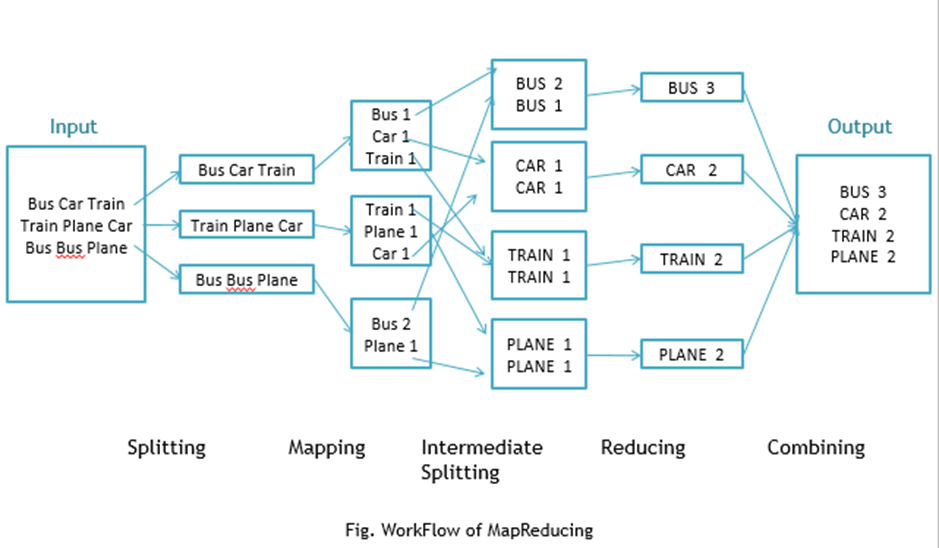
\includegraphics[width=\textwidth,height=\textheight,keepaspectratio]{fig/111.png}
\section{Implementation}
Hadoop streaming is a utility that comes with the Hadoop distribution. The utility allows you to create and run Map/Reduce jobs with any executable or script as the mapper and/or the reducer.For this problem will use Apache Hadoop and ultilize Hadoop streaming to run my mapper and reducer which is written on python language.
\section{How they work}
\subsection{Mapper}
'mapper.py'
The mapper is going to read the complete text of 'word\_input' and take out every word and write that output with a value of 1
\subsection{Reducer}
'reducer.py'
The reducer step is going to combine all the duplicate keys and adding up all the values
\subsection{Execution}
\begin{lstlisting}
'cat word\_input | python mapper.py | sort -k1,1 | python reducer.py'
\end{lstlisting}
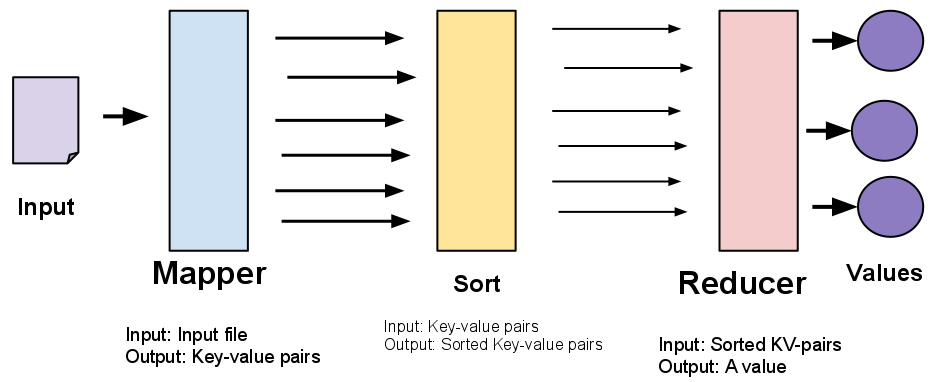
\includegraphics[width=\textwidth,height=\textheight,keepaspectratio]{fig/mapreduce_diag.png}

\end{document}